\chapter{Results}

\section{Pairwise $T^p$ - $T^-$}
From the initial runs where two parameters were changed at a time, the following were observed:
\begin{enumerate}
  %\item $T^p$ is limited by both testosterone and oxygen, whereas $T^-$ is only limited by oxygen. The testosterone limitation is controlled through the two thresholds, $ll_{test,T^p}$ and $ul_{test,T^p}$ as shown in \autoref{freseq}.
  \item Only when $T^p$ is not severely testosterone limited ($ul_{test,T^p}$ is low), $T^p$ can coexist with or outcompete $T^-$ as shown in \autoref{fig_Tpro-Tneg_testlims}. In every other case, $T^-$ drives $T^p$ to extinction.
  \item These competitive outcomes are also dependent on the initial proportion of $T^p$, all the other parameters being the same as shown in  \autoref{fig_Tpro-Tneg_testlims}.
  \item  When $T^-$ is strongly oxygen-limited ($ll_{O_2,T^-} \geq 0.6$) but $T^p$ is also limited by testosterone. In this case, $T^-$ wins out eventually as oxygen levels rise faster than testosterone through the external supply term, $p_{O_2}$ as shown in \autoref{fig_Tpro-Tneg_o2lims}.
  \item When $T^-$ is oxygen limited but with poor oxygen production (lower $p_{O_2}$), $T^p$ is able to drive $T^-$ to extinction as $T^p$ can grow and consume enough oxygen to keep the oxygen levels below those required for $T^-$ to grow as shown in \autoref{fig_Tpro-Tneg_o2lims}.
\end{enumerate}

\begin{figure}[h!]
  \centering
  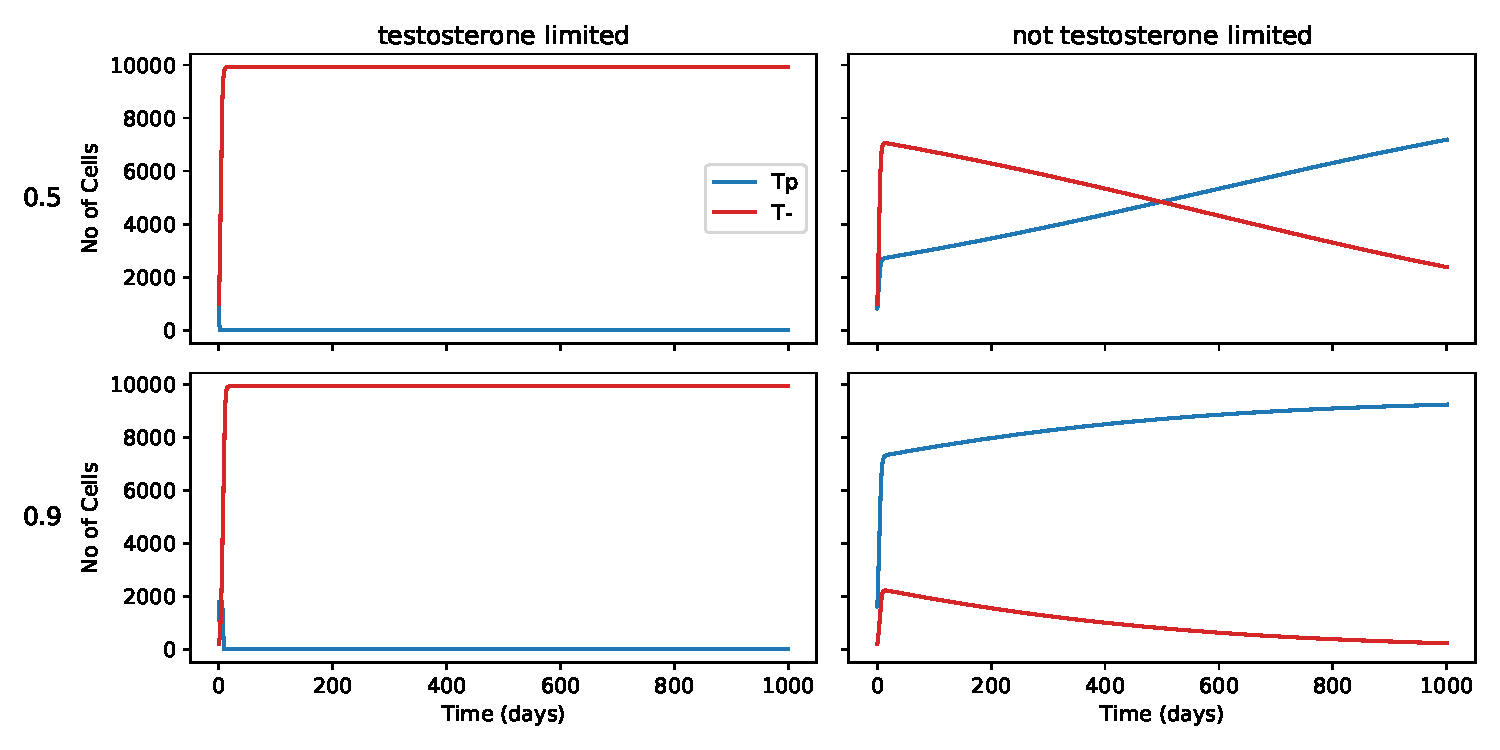
\includegraphics[width=\textwidth]{Tpro-Tneg_testlims}
  \caption[Pairwise $T^p - T^-$ timeseries, testosterone limitation]{Pairwise $T^p - T^-$ timeseries, when $T^p$ is testosterone limited and not testosterone limited (columns) and at different initial proportions of $T^p$ (rows). $T^p$ is testosterone limited at $ul_{test,T^p}=0.5$ and not testosterone limited at $ul_{test,T^p}=0.1$.}
  \label{fig_Tpro-Tneg_testlims}
\end{figure}

\begin{figure}[h!]
  \centering
  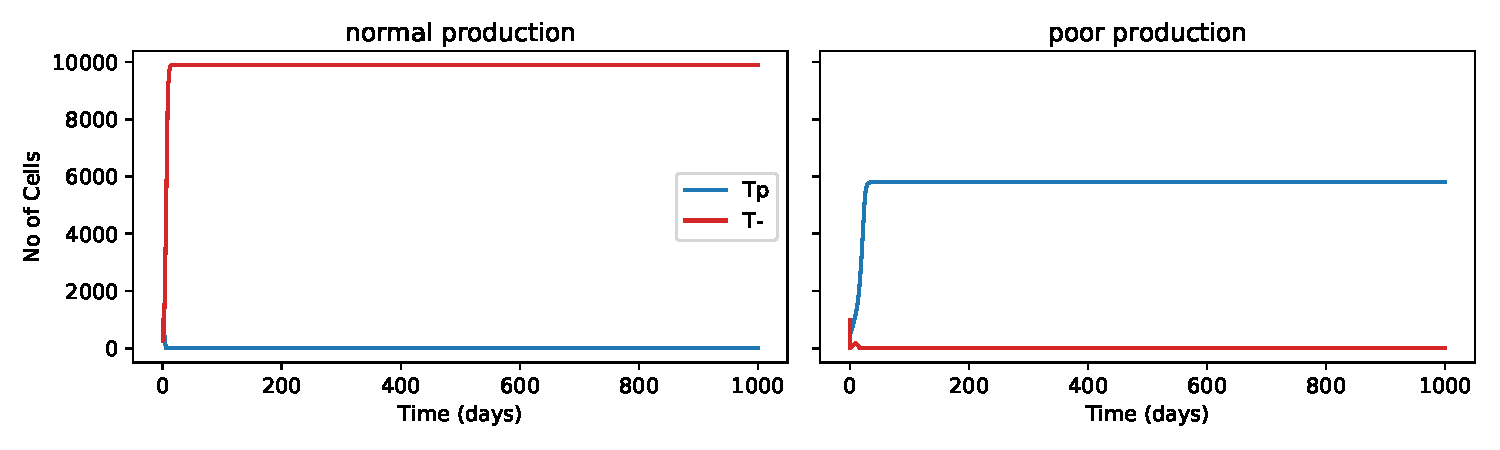
\includegraphics[width=\textwidth]{Tpro-Tneg_o2lims}
  \caption[Pairwise $T^p - T^-$ timeseries, oxygen limitation]{Pairwise $T^p - T^-$ timeseries, when $T^-$ is oxygen limited and at different oxygen production (column). $T^-$ is oxygen limited at $ll_{O_2,T^-}=0.6$ and $T^p$ is testosterone limited at $ul_{test,T^p}=0.5$. The normal and poor production of oxygen are 0.11 and 0.0675 min$^{-1}$ respectively}
  \label{fig_Tpro-Tneg_o2lims}
\end{figure}

Additionally, a brute force parameter space exploration was done over a large combination of parameters. Due to the large parameter set, interpreting the results is difficult and only a few generalised observations were found, as listed below.
\begin{enumerate}
  \item $T^-$ drives $T^p$ to extinction when $ll_{O_2,T^p} \geq 0.6$, regardless of the other parameters, in other words, $T^p$ shouldn't be limited by oxygen to compete with $T^-$. This is visualised in \autoref{fig_Tpro-Tneg_llo2Tp}.
  \item $T^-$ drives $T^p$ to extinction when $ll_{test,T^p} \geq 0.2$, regardless of the other parameters, in other words, $T^p$ needs to be able to grow even on the smallest amount of testosterone to compete with $T^-$. This is visualised in \autoref{fig_Tpro-Tneg_lltestTp}.
  \item $T^-$ drives $T^p$ to extinction when $ul_{test,T^p} \geq 0.3$ and $ll_{O_2,T^-} \leq 0.4$ but not when $ll_{O_2,T^-} \geq 0.6$, in other words, $T^p$ shouldn't be testosterone limited when $T^-$ is not oxygen limited to be to compete with $T^-$. The $ul_{test,T^p}$ required for $T^p$ to not go extinct also increases with increased $ll_{O_2,T^-}$, that is, $T^p$ can afford to be more testosterone limited as $T^-$ becomes more oxygen limited. This is visualised in \autoref{fig_Tpro-Tneg_ultestTp}.
\end{enumerate}

\begin{figure}[h!]
  \centering
  \begin{subfigure}[b]{0.45\textwidth}
    \centering
    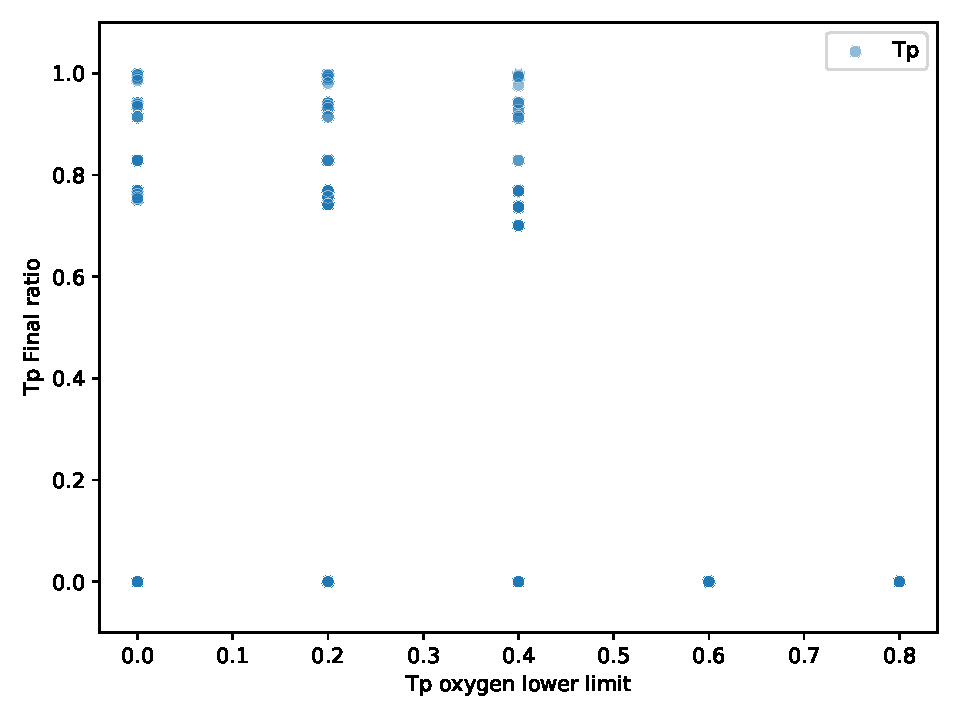
\includegraphics[width=\textwidth]{Tpro-Tneg_llo2Tp}
    \caption{Lower limit of oxygen for $T^p$}
    \label{fig_Tpro-Tneg_llo2Tp}
  \end{subfigure}
  \begin{subfigure}[b]{0.45\textwidth}
    \centering
    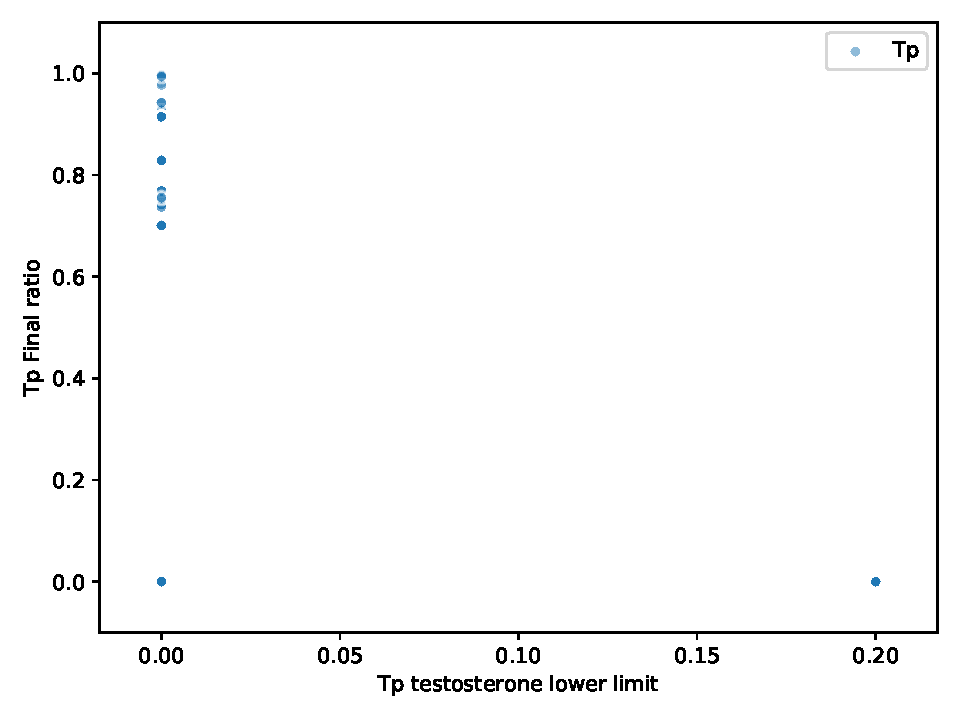
\includegraphics[width=\textwidth]{Tpro-Tneg_lltestTp}
    \caption{Lower limit of testosterone for $T^p$}
    \label{fig_Tpro-Tneg_lltestTp}
  \end{subfigure}
  \begin{subfigure}[b]{0.45\textwidth}
    \centering
    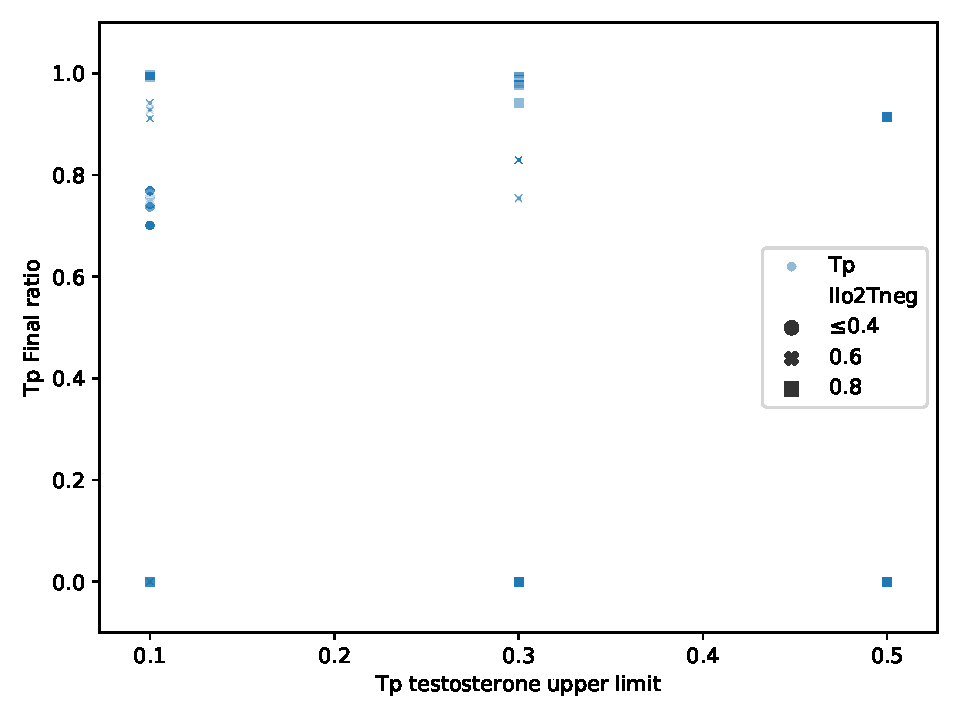
\includegraphics[width=\textwidth]{Tpro-Tneg_ultestTp}
    \caption{Upper limit of testosterone for $T^p$}
    \label{fig_Tpro-Tneg_ultestTp}
  \end{subfigure}
  \caption[Final $T^p$ ratio of pairwise $T^p - T^-$ runs vs parameters]{Final $T^p$ ratio of pairwise $T^p - T^-$ runs vs parameters. Note: The multiple points for same x-value represents values on varying the other parameters.}
  \label{fig_Tpro-Tneg_megarun}
\end{figure}


From the above observations, the following cases were formulated as an exhaustive formulation of possible conditions. Three levels of testosterone limitation of $T^p$
pairwise competitive runs were done over varying initial cell seeding.
\begin{longtable}[c]{|l|l|l|l|}

  \hline \multicolumn{1}{|c|}{\textbf{Case}} & \multicolumn{1}{c|}{\textbf{$O_2$ production}} & \multicolumn{1}{c|}{\textbf{$T^-\ O_2$ limitation}} & \multicolumn{1}{c|}{\textbf{$T^p\ test$ limitation}}\\ \hline
  \endhead

  \hline \multicolumn{4}{|r|}{{Continued on next page}} \\ \hline
  \endfoot

  \endlastfoot

  AAA & normal & no & no \\ \hline
  AAB & normal & no & moderate \\ \hline
  AAC & normal & no & severe \\ \hline
  ABA & normal & high & no \\ \hline
  ABB & normal & high & moderate \\ \hline
  ABC & normal & high & severe \\ \hline
  ACA & normal & severe & no \\ \hline
  ACB & normal & severe & moderate \\ \hline
  ACC & normal & severe & severe \\ \hline
  BAA & poor & no & no \\ \hline
  BAB & poor & no & moderate \\ \hline
  BAC & poor & no & severe \\ \hline
  BBA & poor & high & no \\ \hline
  BBB & poor & high & moderate \\ \hline
  BBC & poor & high & severe \\ \hline
  BCA & poor & severe & no \\ \hline
  BCB & poor & severe & moderate \\ \hline
  BCC & poor & severe & severe \\ \hline

  \caption{Table of cases for $T^p$ - $T^-$ pairwise}
  \label{tab_Tpro-Tneg_cases}
\end{longtable}

Here,
\begin{itemize}
  \item For $O_2$ production: normal and poor correspond to $p_{O_2}=0.11, 0.0675$ min$^{-1}$ respectively.
  \item For $T^-\ O_2$ limitation: no, high and severe correspond to $ll_{O_2,T^-}=0, 0.6, 0.8$ respectively.
  \item For $T^p\ test$ limitation: no, moderate and severe correspond to $ul_{test,T^p}=0.1, 0.3, 1$ respectively.
\end{itemize}

\begin{figure}[h!]
  \centering
  \begin{subfigure}[b]{\textwidth}
    \centering
    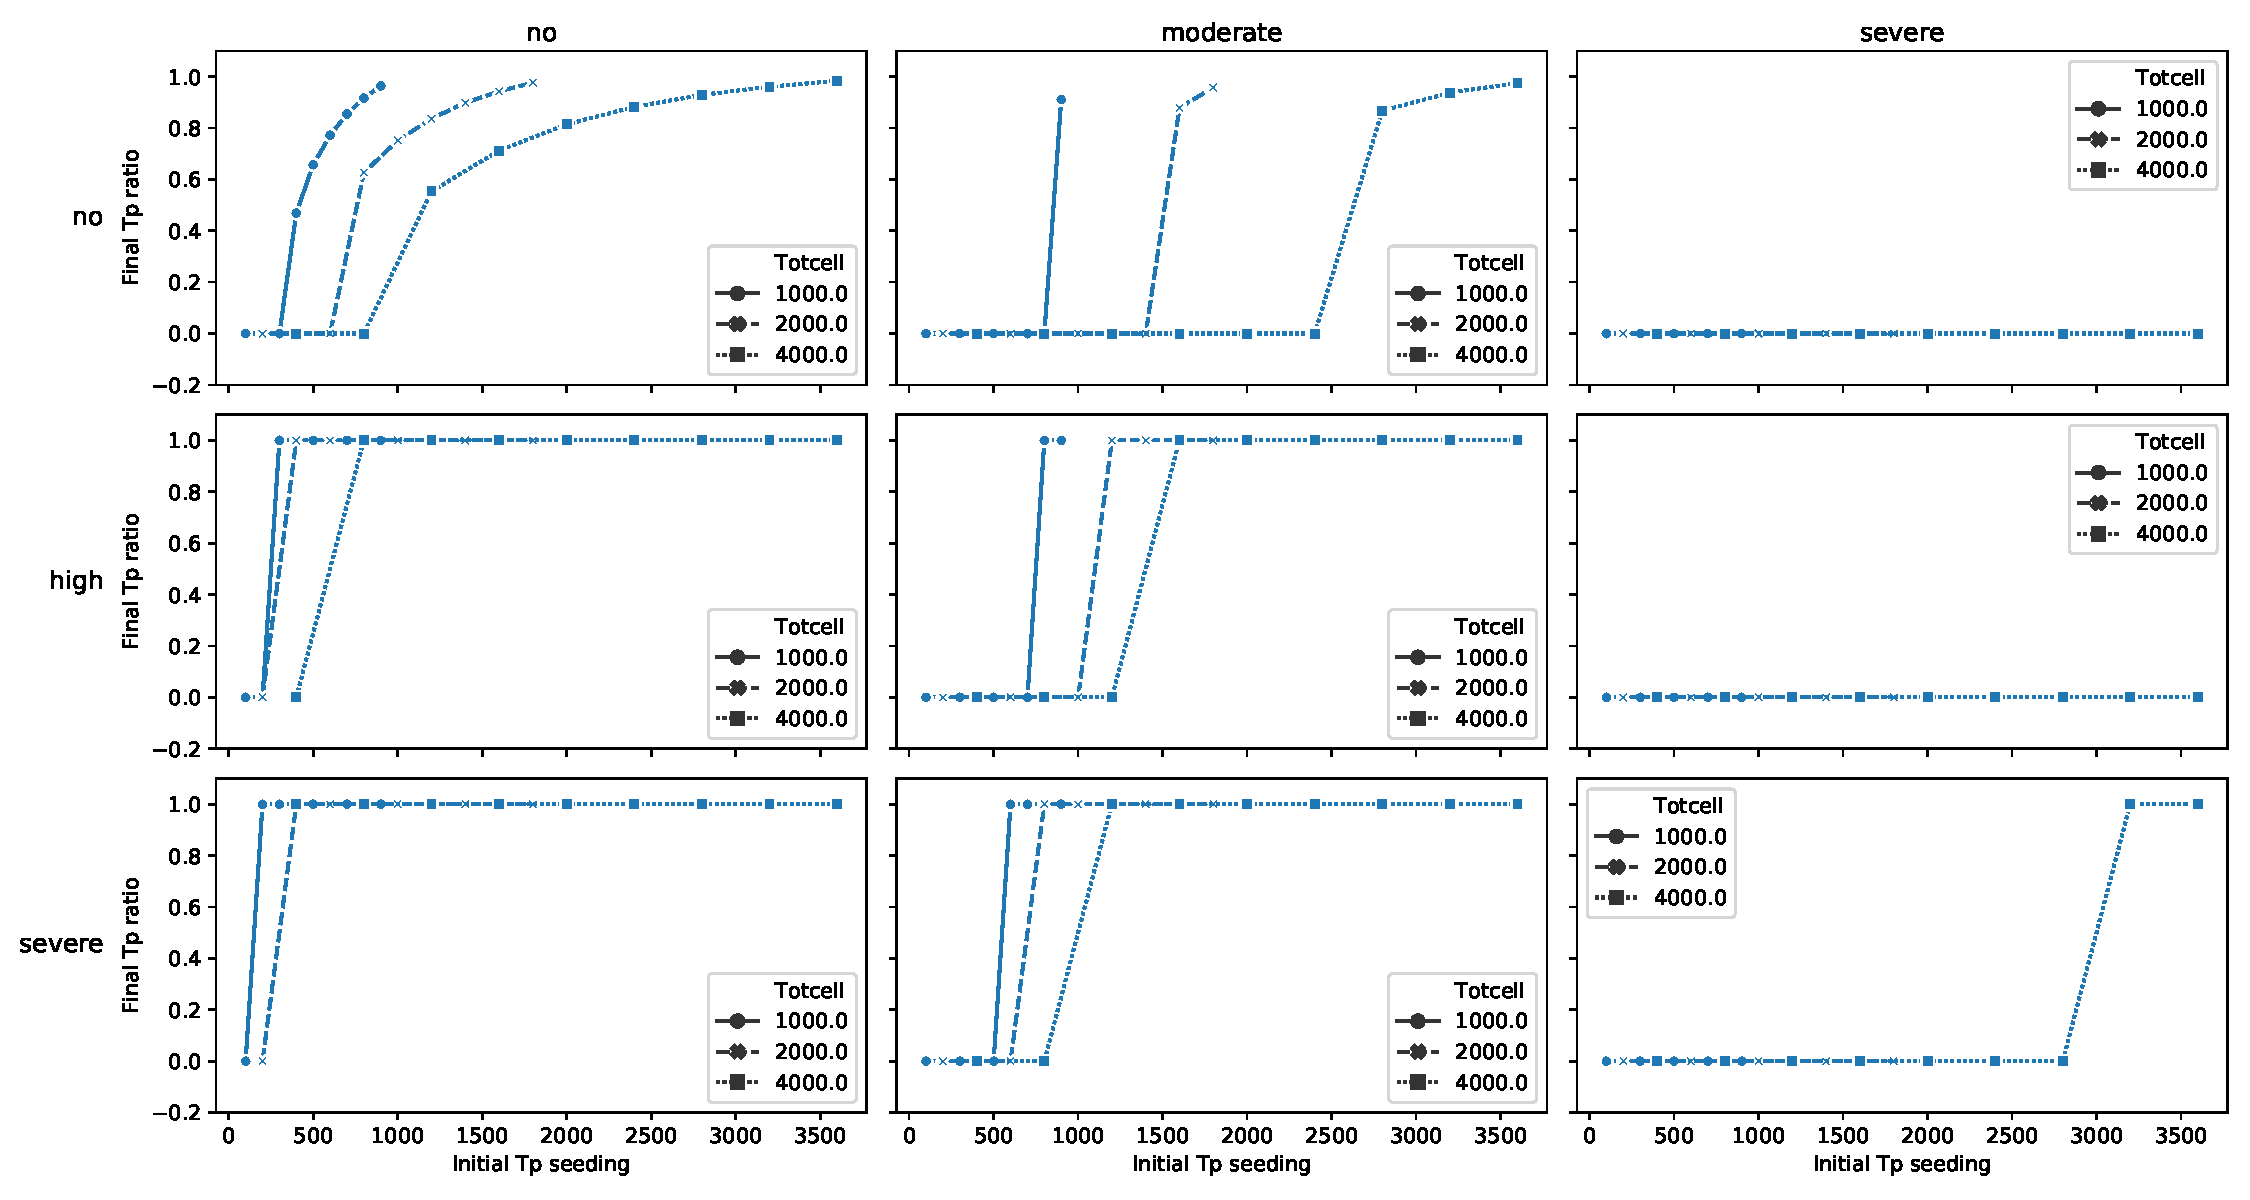
\includegraphics[width=\textwidth]{Tpro-Tneg_cases_normal}
    \caption{normal production}
    \label{fig_Tpro-Tneg_cases_normal}
  \end{subfigure}
  \begin{subfigure}[b]{\textwidth}
    \centering
    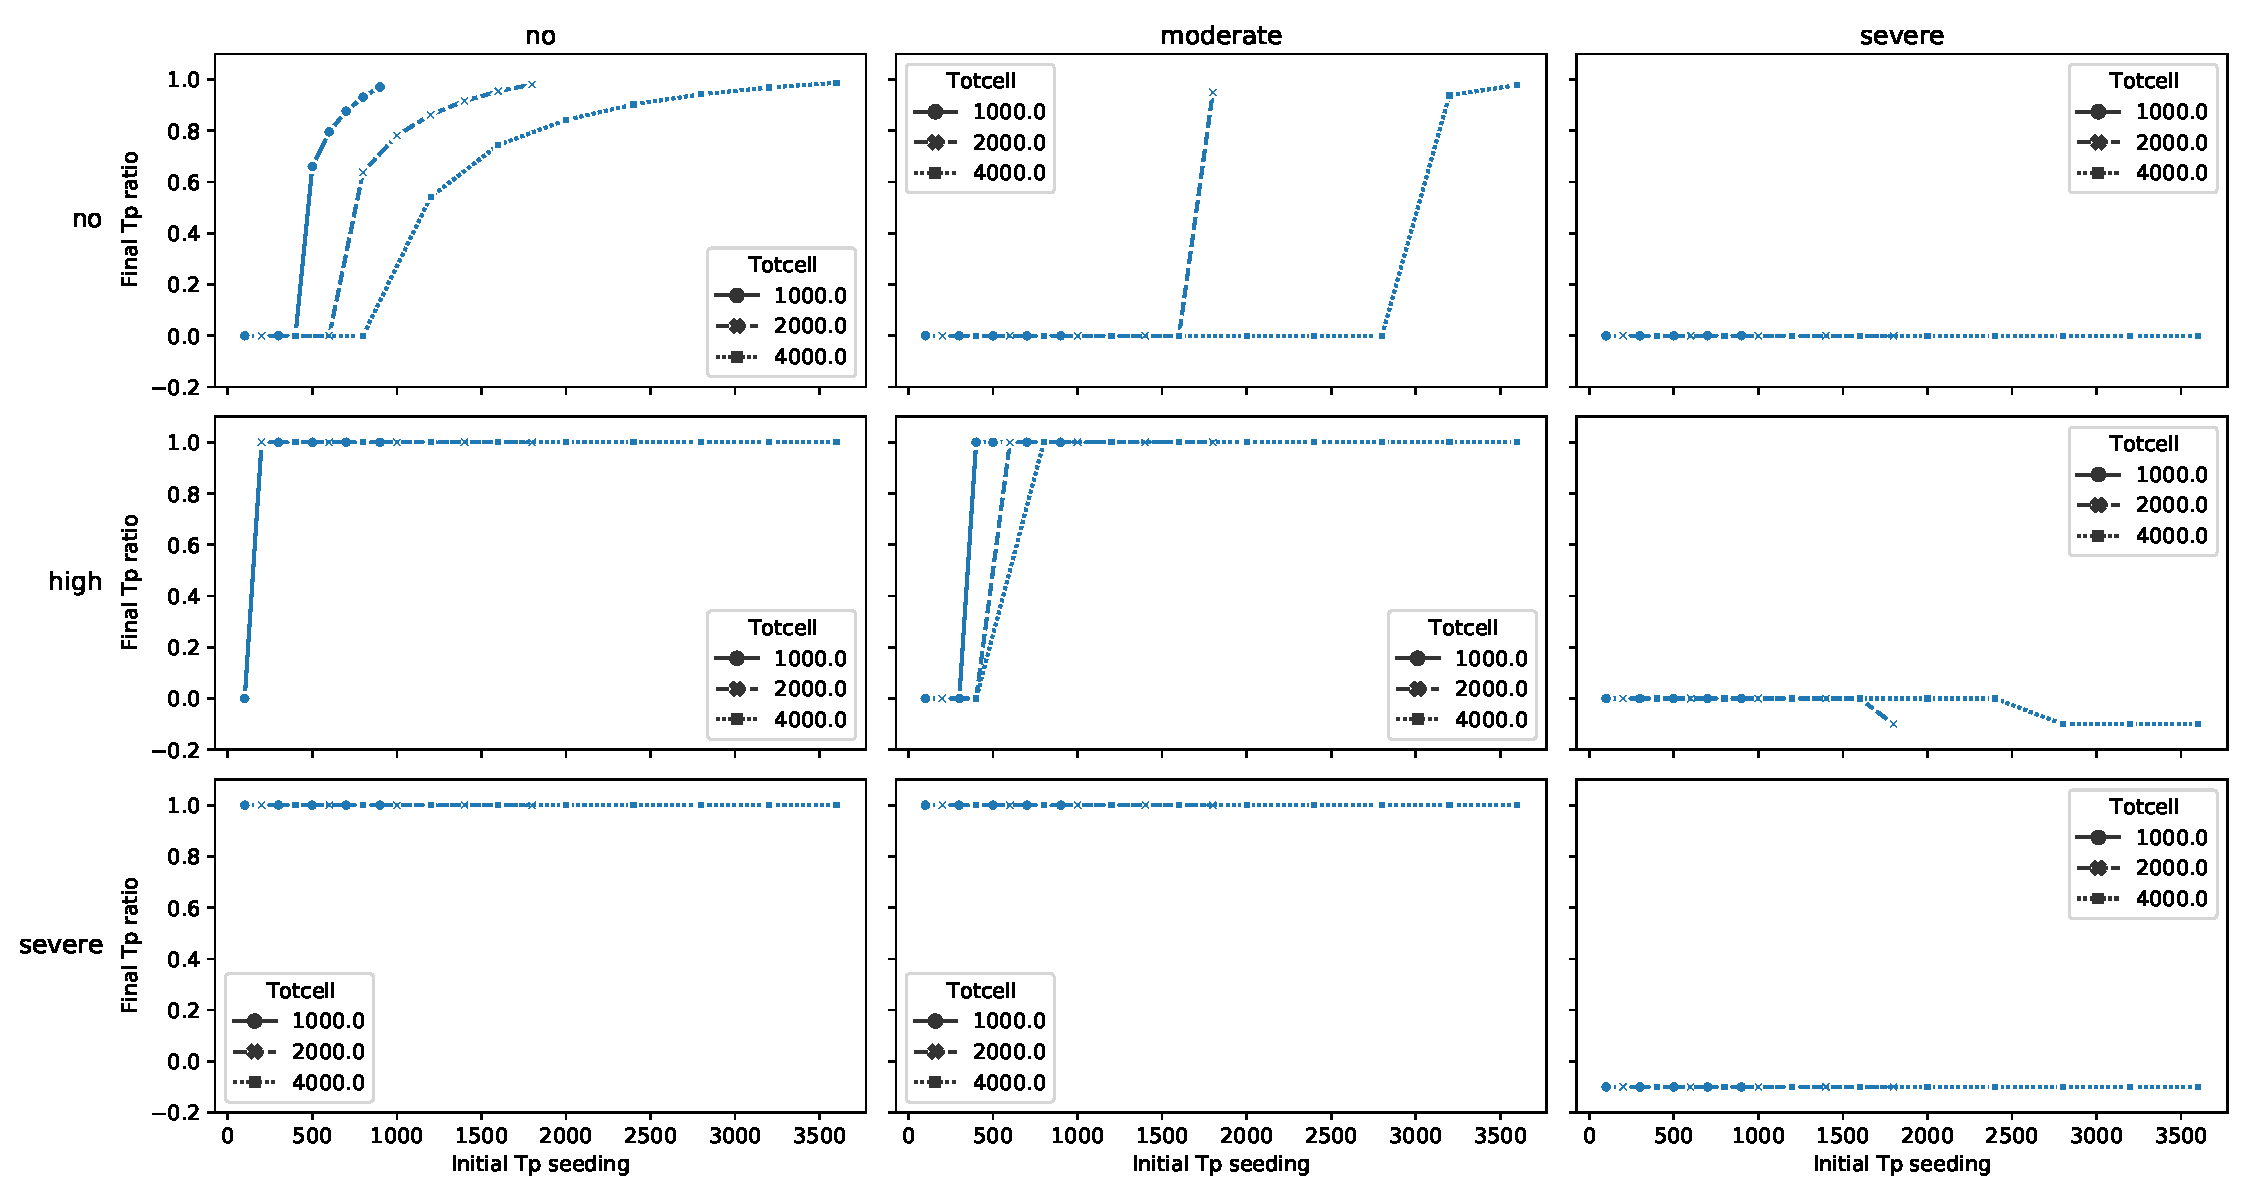
\includegraphics[width=\textwidth]{Tpro-Tneg_cases_poor}
    \caption{poor production}
    \label{fig_Tpro-Tneg_cases_poor}
  \end{subfigure}
  \caption[Final $T^p$ ratio of pairwise $T^p - T^-$ runs under different cases]{Final $T^p$ ratio of pairwise $T^p - T^-$ runs under different cases. Subfigures: $O_2$ Production, Rows: $T^-\ O_2$ limitation, Columns: $T^p\ test$ limitation. Note: Ratio = -0.1 is used when both cell types go extinct.}
  \label{fig_Tpro-Tneg_cases}
\end{figure}

\newpage
The following were observed from the cases as visualised in \autoref{fig_Tpro-Tneg_cases}:
\begin{enumerate}
  \item Coexistence is observed only in cases AAA, AAB, BAA and BAB. All of them have low or moderate limitation of testosterone for $T^p$ and have no limitation of oxygen for $T^-$. For low $T^p$ initial seeding, $T^-$ dominates over $T^p$ and causes it to go extinct, but as $T^p$ initial seeding increases the favour shift towards $T^p$.
  \item $T^-$ causes $T^p$ to go extinct for all initial seedings in cases AAC, ABC, BAC and BBC. $T^p$ is severely testosterone limited and even with a high initial seeding advantage, $T^-$ grows, overtakes $T^p$ and eventually causes $T^p$ to go extinct. At high $T^p$ initial seeding, $T^-$ also goes extinct in case BBC due to high oxygen limitation on it.
  \item The outcome switches from $T^p$ going extinct to $T^-$ going extinct for higher $T^p$ initial seeding in cases ABA, ABB, ACA, ACB, ACC, BBA and BBB. As with cases AAA, AAB, BAA and BAB, for low $T^p$ initial seeding, $T^-$ dominates over $T^p$ and causes it to go extinct, but as $T^p$ initial seeding increases the favour shift towards $T^p$. However, in this case the oxygen levels don't go above the levels required for $T^-$ to grow before it goes extinct and only $T^p$ remains. Case ACC has this switch only at the highest $T^p$ initial seeding as it is also severely testosterone limited.
  \item $T^-$ goes extinct for all initial seedings in cases BCA, BCB and BCC. $T^p$ also goes extinct in the case BCC. The oxygen limitation on $T^-$ is too high and the oxygen levels never reach the levels required for a non-zero growth for $T^-$. In the case BCC, $T^p$ is weighed down by both the testosterone limitation and density-dependent competition of the remaining $T^-$ cells and goes extinct as a result.
\end{enumerate}

\section{Pairwise $T^+$ - $T^p$}
From the initial runs where two parameters were changed at a time, the following were observed:
\begin{enumerate}
    %\item Both $T^+$ and $T^p$ are limited by both oxygen and testosterone, and compete for both resources. As with the other pair, strength of limitation for any particular resource can be modulated through the corresponding upper and lower thresholds.
    \item When $T^p$ limited by testosterone more than $T^+$ ($ul_{test,Tp} > ul_{test,T+}$), $T^+$ can consume and grow on the limited testosterone present, and this is enough for the density-dependent competition to drive $T^p$ to extinction. Without $T^p$ to provide testosterone, $T^+$ subsequently goes extinct.
    \item When $T^p$ is weakly limited by testosterone relative to $T^+$ ($ul_{test,Tp} \leq ul_{test,T+}$), both cells coexist. Due to weaker testosterone limitation, $T^p$ can grow faster initially and secrete enough testosterone for $T^+$ without being negatively affected by $T^+$. This is visualised in \autoref{fig_Tpos-Tpro_testlims}.
    \item In the above case, the proportion of $T^+$ in the final population decreases as $T^+$ becomes more testosterone limited.
    \item When both are severely testosterone limited but not oxygen limited, $T^p$ causes $T^+$ to go extinct. However, in a special scenario when both are oxygen limited with $T^+$ being more limited, coexistence is observed. A balance of sort is achieved here, where, in the initial period of low oxygen, $T^p$ can grow more than $T^+$ and secrete enough testosterone to sustain both population but doesn't grow as much as to drive $T^+$ to extinction. This is visualised in \autoref{fig_Tpos-Tpro_o2lims}.
  \end{enumerate}

\begin{figure}[h!]
  \centering
  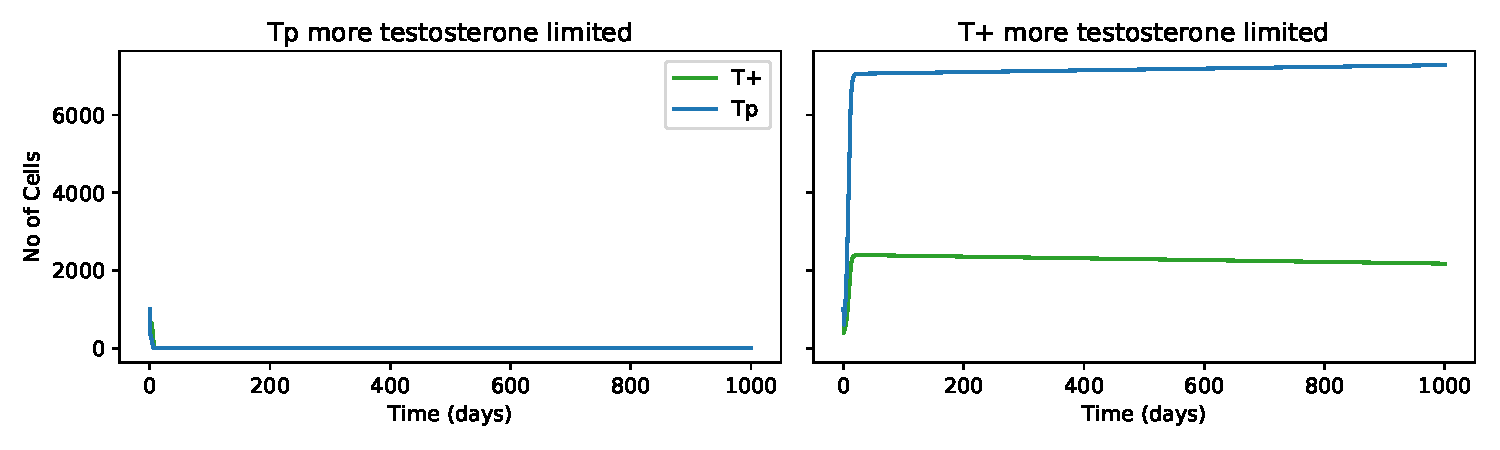
\includegraphics[width=\textwidth]{Tpos-Tpro_testlims}
  \caption[Pairwise $T^+ - T^p$ timeseries, testosterone limitation]{Pairwise $T^+ - T^p$ timeseries, when $T^p$ is more testosterone limited than $T^p$ and when $T^+$ is more testosterone limited than $T^p$. $T^p$ is more limited testosterone limited at $ul_{test,T^+}=0.3,ul_{test,T^p}=0.5$ and $T^+$ is limited more at $ul_{test,T^+}=0.5,ul_{test,T^p}=0.3$.}
  \label{fig_Tpos-Tpro_testlims}
\end{figure}

\begin{figure}[h!]
\centering
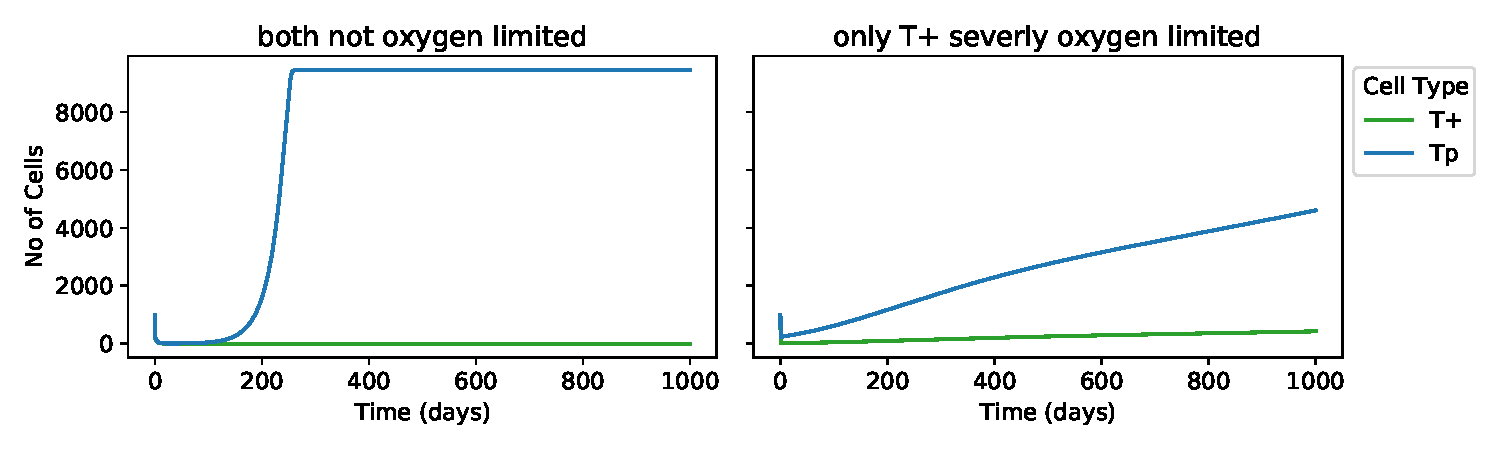
\includegraphics[width=\textwidth]{Tpos-Tpro_o2lims}
\caption[Pairwise $T^+ - T^p$ timeseries, oxygen limitation]{Pairwise $T^+ - T^p$ timeseries, when both cell types are testosterone limited and not oxygen limited at $ll_{O_2,T^+}=0.0, ll_{O_2,T^p}=0.0$ and $T^+$ is oxygen limited and $T^p$ moderately at $ll_{O_2,T^+}=0.6, ll_{O_2,T^p}=0.4$.}
\label{fig_Tpos-Tpro_o2lims}
\end{figure}

From the above observations, the following cases were formulated as representative and pairwise competitive runs were done over varying initial cell seeding.

\begin{longtable}[c]{|l|l|l|l|l|}

  \hline \multicolumn{1}{|c|}{\textbf{Case}} & \multicolumn{1}{c|}{\textbf{$T^+\ test$ limitation}} & \multicolumn{1}{c|}{\textbf{$T^+\ O_2$ limitation}} & \multicolumn{1}{c|}{\textbf{$T^p\ test$ limitation}} & \multicolumn{1}{c|}{\textbf{$T^p\ O_2$ limitation}} \\ \hline
  \endhead

  \hline \multicolumn{3}{|r|}{{Continued on next page}} \\ \hline
  \endfoot

  \endlastfoot
  1 & no & no & moderate & no \\ \hline
  2 & moderate & no & no & no \\ \hline
  3 & severe & high & severe & moderate \\ \hline
  4 & severe & high & severe & no \\ \hline
  \caption{Table of cases for $T^+$ - $T^p$ pairwise}
  \label{tab_Tpro-Tneg_cases}

\end{longtable}

Here, for $T^+/T^p\ test$ limitation: no and moderate correspond to $ll_{O_2,T^i}=0.1, 0.3$ respectively.

\begin{figure}[h!]
  \centering
  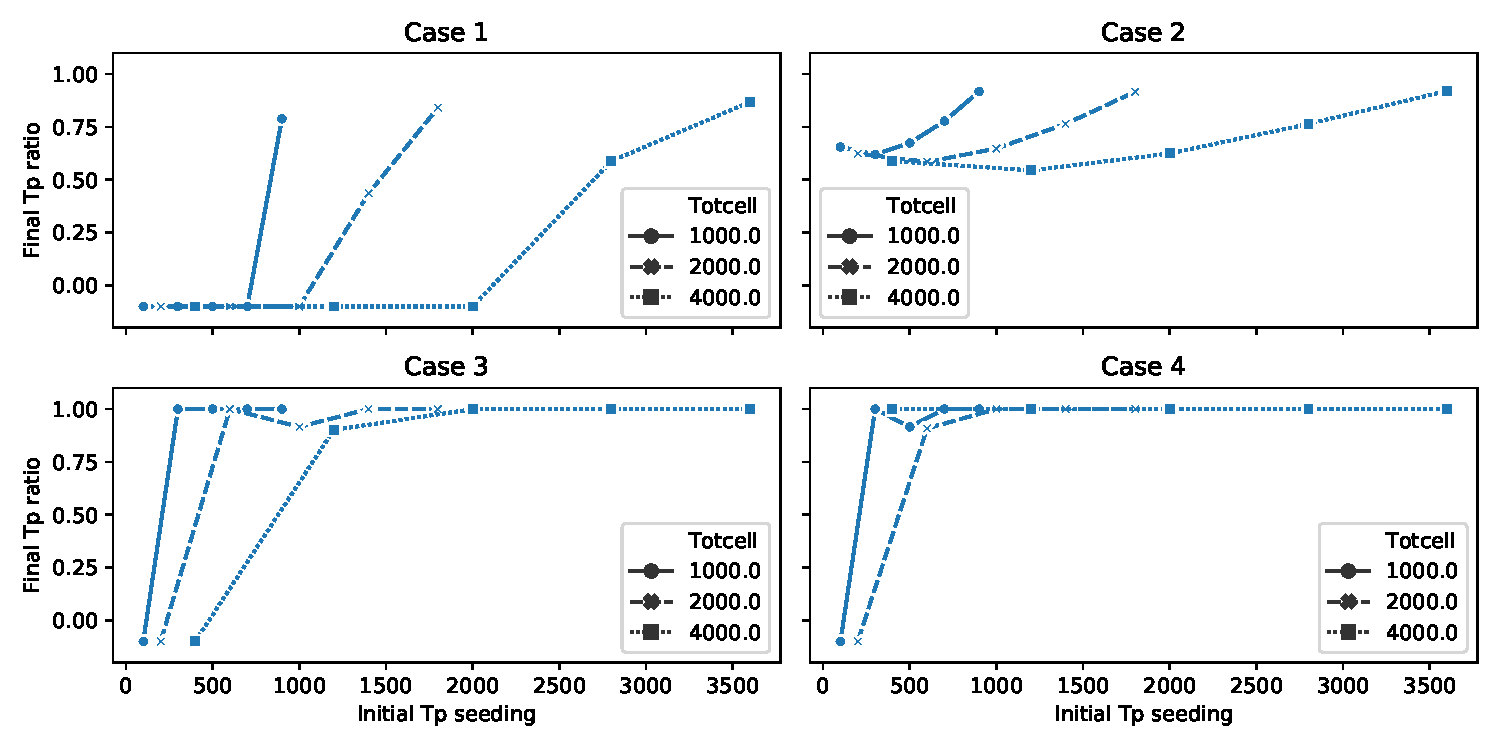
\includegraphics[width=\textwidth]{Tpos-Tpro_cases}
  \caption[Final $T^p$ ratio of pairwise $T^+ - T^p$ runs under different cases]{Final $T^p$ ratio of pairwise $T^+ - T^p$ runs under different cases. Case 1: $T^+$ is not testosterone limited and $T^p$ is moderately testosterone limited, Case 2: $T^+$ is moderately testosterone limited and $T^p$ is not testosterone limited. Note: Ratio = -0.1 is used when both cell types go extinct.}
  \label{fig_Tpos-Tpro_cases}
\end{figure}

\newpage
The following were observed from the cases as visualised in \autoref{fig_Tpro-Tneg_cases}:
\begin{enumerate}
  \item  In case 1, both the cell types go extinct when $T^p$ has low initial seeding as seen previously, whereas at high $T^p$ initial seeding, both are able to coexist. At high $T^p$ initial seeding, $T^p$ is able to grow without density-dependent suppression by $T^+$ and secrete more testosterone from their higher overall number despite being disadvantaged in their growth compared to $T^+$.
  \item In case 2, both cells are able to coexist at all $T^p$ initial seeding. However, there exists a sweet spot for $T^+$ where it has the maximum final ratio. At high $T^p$ initial seeding, $T^p$ suppresses $T^+$ from growing through its large number, whereas, at very low $T^p$ initial seeding, $T^+$ needs $T^p$ to grow for its testosterone.
  \item In case 3, at low $T^p$ initial seeding, both cell types go extinct as $T^+$ due to it’s higher number consumes the testosterone produced by $T^p$ and doesn’t let it grow. However, at higher $T^p$ seeding, $T^+$ goes extinct as $T^+$ cannot grow due to oxygen limitation before being suppressed by $T^p$. Only at intermediate $T^p$ seeding do both coexist as both of them inhibit each other for oxygen.
  \item Case 4 is very similar to Case 3, however, the intermediate $T^p$ seeding at which they coexist is lower.  Since, $T^p$ is not oxygen limited, it can grow more easily compared to Case 3 for the same initial $T^p$ seeding and can outcompete $T^+$ more easily.
\end{enumerate}
